
\item Se o coeficiente de atrito cinético entre a caixa de \SI{100}{\kilogram} e o plano 
é $\mu_{k}=0.25$, determine a velocidade da caixa no instante que a compressão da mola é $x=\SI{1.5}{\meter}$. Inicialmente, a mola não está deformada e a caixa está em repouso.

\import{answers/}{answer-8}

\vspace{-1.5cm}
\begin{flushright}
    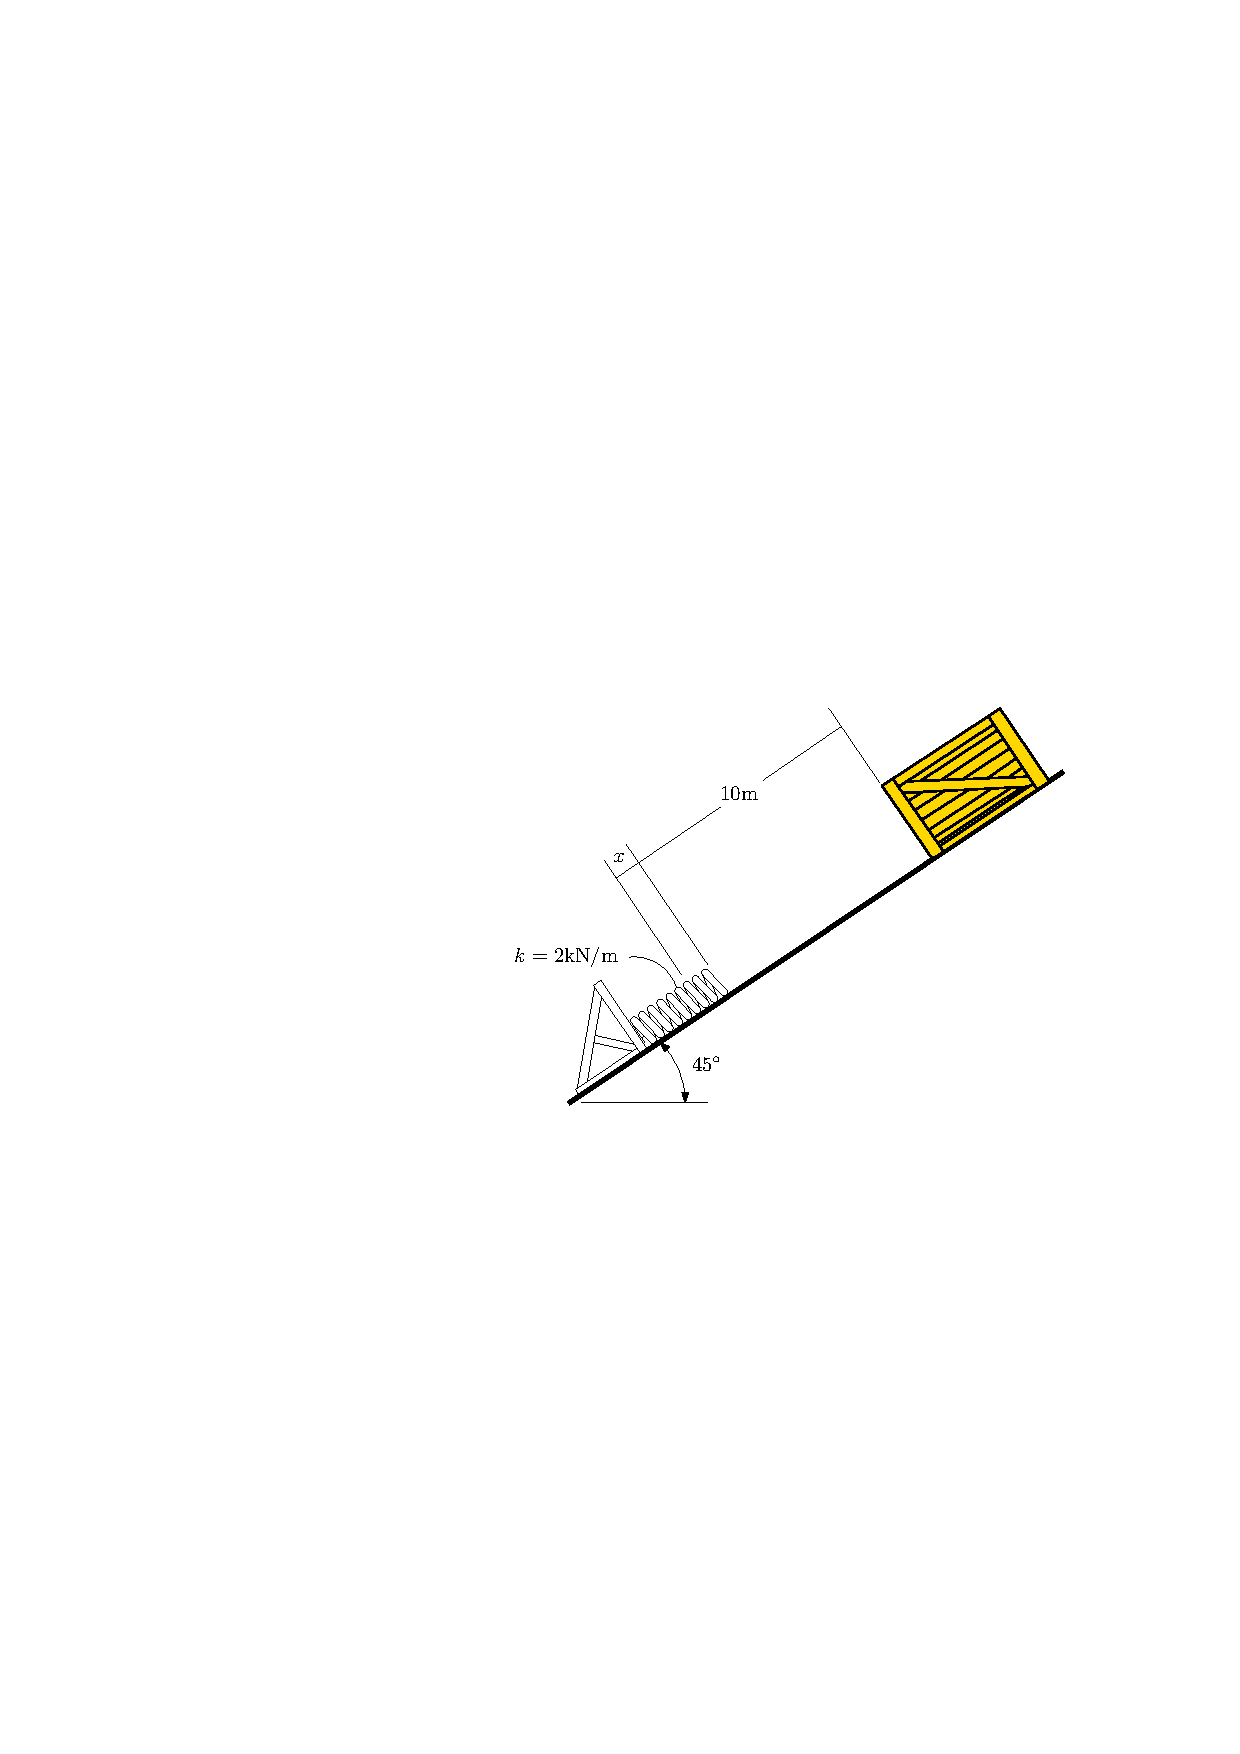
\includegraphics[scale=1.3]{images/draw_8.pdf}
\end{flushright}